\documentclass[a4paper,12pt]{report}
\usepackage{graphicx}
\usepackage{titlesec}
\titleformat{\chapter}{}{}{0em}{\bf\LARGE}
\usepackage[utf8]{inputenc}
% Title Page
\title{Middle East Technical University\\Department of Physics\\PHYS222 Optics and Waves Laboratory\\\textbf{Experiment OW-8\\Microwave Optics 2\\Laboratory Report}}

\author{Oğuzhan ÖZCAN\\1852334\\\\Partner: İnci SAİM\\\\Teaching Assistant: Hikmet ÖZŞAHİN}


\begin{document}
\maketitle
\tableofcontents
\listoffigures
\listoftables
\chapter{Theory}
Microwaves are a form of electromagnetic radiation. The microwave band extends from 300 MHz to 300 GHz. In this gap there are some specified bands. The frequency range from 300 MHz to 3 GHz is called the ultra high frequency (UHF) band, from 3 GHz to 30 GHz is super high frequency (SHF) band and from 30 GHz to 300 GHz is the extremely high frequency (EHF) band. These three frequency range comes together and make microwave band spectrum. Note that there are spectrums for different wavelengths (See Figure 1.1).
\begin{figure}[h]
\centering
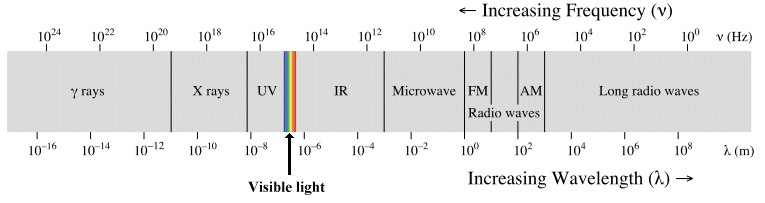
\includegraphics[width=1.0\linewidth, height=0.22\textheight]{spectrum}
\caption{Wavelength Spectrum}
\label{fig:spectrum}
\end{figure}
Applications of microwaves are varies. For instance military radars are operate at 450 MHz, UHF brodcast TV operates at 470-870 MHz, cellular telephone band operates at 900 MHz and air traffic radar operates at above 1 GHz [1].\\\\
Since microwave is an electromagnetic wave it has electric field $\vec{E}$ and magnetic field $\vec{B}$. These components are perpendicular to each other (See Figure 1.2). Relationship between electric field and magnetic field can described by using speed of light as follows
\begin{center}
	{\large $c=\frac{E}{B}$}
\end{center}
An important topic about waves is standing waves or also known as stationary waves.
\begin{figure}[h]
\centering
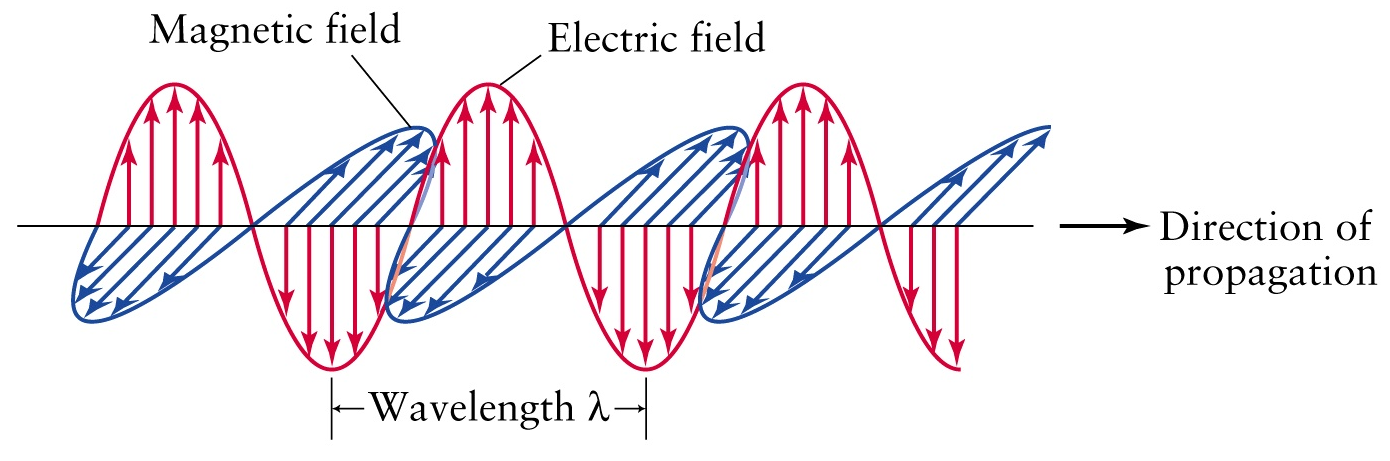
\includegraphics[width=1.0\linewidth, height=0.23\textheight]{em}
\caption{Components of Electromagnetic Wave}
\label{fig:em}
\end{figure}
When two harmonic waves of the same frequency propagating in opposite direction these waves called as standing waves. If we examine an example situation let we have an incident wave which is reflected backward from a rigid wall. Incoming wave travelling to left and reflected wave travelling to right. The two waves exists simultaneously in the region between the source and mirror. The two overlapping waves would have to add each other and yield a zero resultant wave. This situation is related to \textit{boundary conditions} [2]. If we want to describe this situation with mathematics, we will have two different equations for right incident wave and left incident wave.
\begin{center}
	$E_{L}=E_{0L}\sin(kx+\omega t+\epsilon_{L})$\\
$E_{R}=E_{0R}\sin(kx-\omega t+\epsilon_{R})$
\end{center}
When we combine these two equation we will get
\begin{center}
	$E=E_{0L}[\sin(kx+\omega t)+\sin(kx-\omega t)]$
\end{center}
when apply sinus identity this equation yields to 
\begin{center}
	$E(x,t)=2E_{0L}\sin kx \cos \omega t$
\end{center}
which is known as the equation for standing waves. In standing waves there are two important terms: node and antinode. Between the two mirrors, stationary waves are found with fixed minima
(nodes) and maxima (antinodes) where the electric and magnetic fields may
be considerably reinforced [3]. At certain points when the disturbance will be zero always  $x=0$, $\lambda/2$, $3\lambda/2$... these points are known as nodes. Antinodes are located at halfway between each adjacent node which is at $x=\lambda/4$, $ 3 \lambda/4$, $5 \lambda/4$...
(See Figure 1.3).
\begin{figure}[h]
\centering
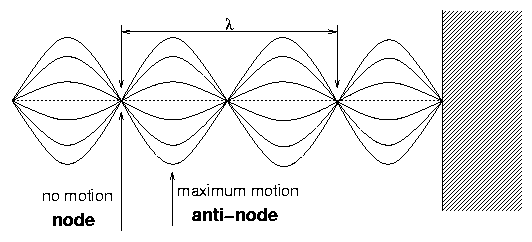
\includegraphics[width=0.85\linewidth, height=0.21\textheight]{standing2}
\caption{Standing (Stationary) Waves}
\label{fig:standing2}
\end{figure}
We can demonstrate standing waves when we direct microwaves onto a metal sheet. The standing wave pattern produced by a 10 cm wavelength source will have nodes spaced 5 cm apart, which are readily observed using a diode detector [4]. Formation of standing waves first observed by Otto Wiener in 1890 and in literature this observation known as \textit{Wiener's Experiment} (See Figure 1.4) [5]. Wiener demonstrated the formation of standing waves of light by reflection from a silver mirror.
Wiener also used his arrangement to examine the interference effects when the angle of incidence is $45^{\circ}$ and the incident light is linearly polarized [6]. When use a metal reflector with a polarization grill we can produce circularly polarized light. 
\begin{figure}[h]
\centering
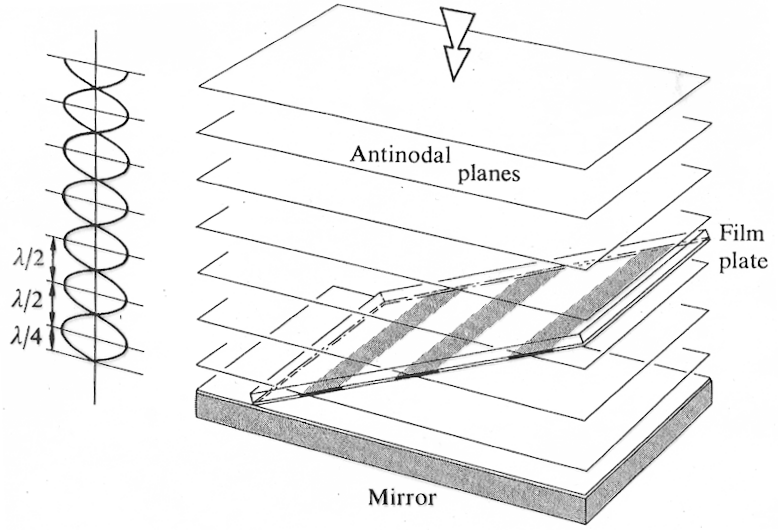
\includegraphics[width=0.7\linewidth, height=0.25\textheight]{wiener}
\caption{Wiener's Experiment Setup}
\label{fig:wiener}
\end{figure}
When the electric field vectors travels around a circle then we have a light beam which is circulary polarized. In this case both waves have same amplitude
\begin{center}
	$E_{0}=E_{0x}=E_{0y}$ 
\end{center}
In this sense the relative phase difference is $\epsilon=-\pi/2+2m\pi$ where \textit{m} is equal to $m=\pm1,\pm2,\pm3,...$ Therefore the electric field equations will be  
\begin{center}
	$\vec{E}_{x}(z,t)=\hat{i}E_{0x}\cos(kz-\omega t)$\\$\vec{E}_{y}(z,t)=\hat{j}E_{0y}\sin(kz-\omega t)$
\end{center}
Thus the resulting wave will be
\begin{center}
	$\vec{E}=E_{0}[\hat{i}\cos(kz-\omega t)+\hat{j}\sin(kz-\omega t)]$
\end{center}
There are two types of circular polarized light: the right-hand circular polarized light and the left-hand circular polarized light. When we look at the electric vector if it as the light comes straight toward us and goes around in a counter-clockwise direction then we call it right-hand circular polarization and the opposite situation called as left-hand circular polarization $[5]$. The circular polarization is a well-known method to give a criterion to distinguish between prolate and oblate crystals $[3]$. When we produce circlularly polarized light with linearly polarized light we use polarizing grills and polaroid filter. By using these filters we can stop the components of electromagnetic waves. A proper filter transmits one or more very narrow bands of wavelength. The separation of the bands produced in the spectrum
by a single crystal is inversely proportional to the thickness of the material [5]. In this manner we we should give some attention to speed of light when passing that kind of filter or materials. In the air, speed of light measured as $2.99\times10^{8}$ m/s. However when we use a material which has a different indices from air, velocity should change. We can define speed of light by using following equation
\begin{center}
{\Large 	$V=\frac{c}{\sqrt{\epsilon}}$}
\end{center}
relationship between $\epsilon$ and indice $n$
\begin{center}
	$n=\sqrt{\epsilon}$
\end{center}
Evidently this relation cannot be rigorously fulfilled, for the reason that the indice depends for all bodies upon the color, i.e. upon the period of oscillation, while from its definition $\epsilon$ is independent of the period of oscillation [7]. 





































\chapter{Data and Results}
\section{Double Slit Interference}
\begin{table}[h]
	\begin{center}
\begin{tabular}{|c|c|c||c|c|c|}
	\hline Angle & Clockwise \textit{I} & C-Clokwise \textit{I} & Angle & Clockwise \textit{I} & C-Clokwise \textit{I} \\ 
	\hline $0^{\circ}$ & 5.4 & 5.0 & $45^{\circ}$ & 0.6 & 1.2 \\ 
	 $5^{\circ}$ & 4.0 & 1.0 & $50^{\circ}$ & 1.0 & 1.2 \\ 
	 $10^{\circ}$ & 0.2 & 0 & $55^{\circ}$ & 0.6 & 1.2 \\ 
	 $15^{\circ}$ & 0.2 & 2.4 & $60^{\circ}$ & 0 & 0.4 \\ 
	 $20^{\circ}$ & 3.4 & 7.8 & $65^{\circ}$ & 0 & 0 \\ 
	 $25^{\circ}$ & 5.0 & 3.2 & $70^{\circ}$ & 0 & 0 \\ 
	 $30^{\circ}$ & 1.0 & 0 & $75^{\circ}$ & 0 & 0 \\ 
	 $35^{\circ}$ & 0 & 0 & $80^{\circ}$ & 0 & 0 \\ 
	 $40^{\circ}$ & 0 & 0.2 & $85^{\circ}$ & 0 & 0 \\ 
	\hline
	\multicolumn{6}{|c|}{\textit{Note: I refers to Intensity Reading }} \\
	\hline 
\end{tabular} 
\end{center}
\caption{Sample Data for Intensity Reading}
\end{table}
\textbf{1. From your data, plot a graph of meter reading versus $\theta$. Identify the angles at which the maxima and minima of the interference pattern occur.}\\\\
\begin{figure}[!h]
\centering
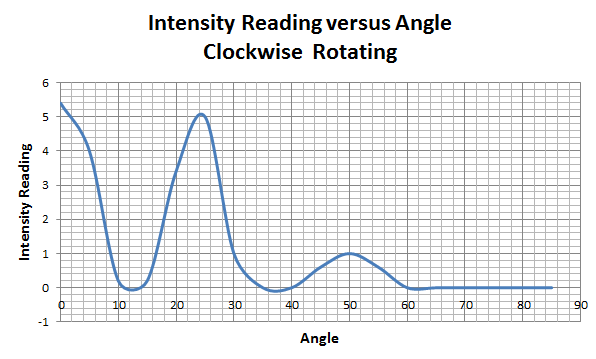
\includegraphics[width=1.0\linewidth, height=0.42\textheight]{clock}
\caption{Intensity Reading vs Angle $\theta$ - Clockwise}
\label{fig:clock}
\end{figure}
\begin{figure}[!h]
\centering
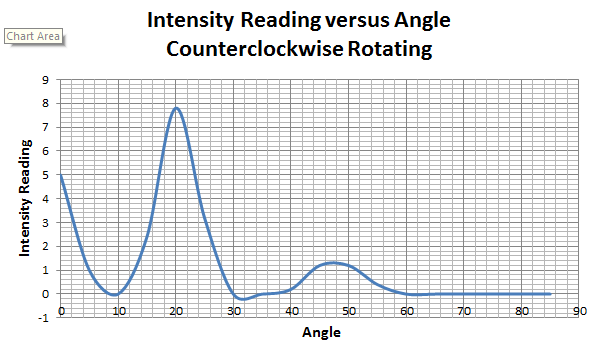
\includegraphics[width=1.0\linewidth, height=0.42\textheight]{c-clock}
\caption{Intensity Reading vs Angle $\theta$ - Counterclockwise}
\label{fig:c-clock}
\end{figure}
In the clockwise rotation we have minimas at the angle of 12.5$^{\circ}$ and 37.5$^{\circ}$ and maximas at the angle of 0.0$^{\circ}$, 25.0$^{\circ}$ and 50.0$^{\circ}$. In the counterclockwise rotation we have minimas at the angle of 10.0$^{\circ}$ and 30.0$^{\circ}$ and besides we have maximas at the angle of 20.0$^{\circ}$ and 47.5$^{\circ}$ (See Figures 2.1 and 2.2).\\\\
\textbf{2. Calculate the angles at which you would expect the maxima and minima to occur in a standard two slit diffraction pattern-maxima occur wherever $d\sin\theta=n\lambda$, minima occur wherever $d\sin\theta=n \lambda/2$ (Check your textbook for the derivation of these equations, and use the wavelength measured in experiment OW-7). How does this compare with the locations of your observed maxima and minima? Can you explain any discrepancies? What assumptions are made in the derivations of the formulas and to what extent are they met in this experiment?}\\\\ 
In the experiment OW-7, we measured the wavelength of the microwave as 0.028 m. There is a small amount of error because PASCO states that wavelength at 10.525 GHz is 2.85 cm [8]. The distance $d$ is 1.5 cm. When we calculate a minima
\begin{center}
	$d\sin\theta=n\lambda/2$
\end{center}
\begin{center}
	$\sin\theta=2.8 cm/3.0cm$ then $\sin\theta=0.95$
\end{center}
Therefore we have a minima at $\theta=\sin^{-1}0.95$ $\theta=71.8^{\circ}$. Since the our experimental results does not support this theoretical value, we cannot make critization about experimental results.\\\\
\textbf{3. Can you explain the relative drop in intensity for higher order maxima? Consider single-slit diffraction pattern created by each slit. How do these single slit patterns affect the overall interference pattern?}\\\\
As we studied in the experiment OW-7, the single-slit pattern acts as an upper limit to the multiple-slit pattern from this experiment.







\newpage
\section{Thin-Film Interference}
\begin{table}[h!]
	\begin{center}
\begin{tabular}{|c|c|c|c|c|c|}
    \hline
    \multicolumn{6}{|c|}{Reflector positions for minima} \\
	\hline 30.0 cm& 26.2 cm& 25.3 cm& 23.2 cm& 21.9 cm& 20.1 cm\\ 
	\hline 
\end{tabular} 
\end{center}
\caption{Sample Data for Minima Positions}
\end{table}
\textbf{1. Is the distance between successive minima or maxima one half the wavelength? Explain why?}\\\\
The distance $x$ can be obtained as
\begin{center}
	$x=\frac{\sum |x_{i+1}-x_{i}|}{N}$
\end{center}
Therefore
\begin{center}
	$x=\frac{|3.8+0.9+2.1+1.3+1.8|}{5}$
\end{center}
\begin{center}
	$x=1.98$ cm
\end{center}
As we know from experiment OW-7, the wavelength is 2.85 cm and its half is 1.425 cm. We found the successive minima as 1.98 cm. Apperantly, we have some experimental error. If we calculate the percentage error we can determine how much wrong data do we have. Thus,
\begin{center}
	Percentage Error=$\frac{|1.425-1.98|}{1.425}\times100\%=38.9\%$
\end{center}

























\chapter{Discussion and Conclusion}
\textbf{1. What are the possible errors in the experiment?}\\
The most possible error cause is diffraction grating since we used slits. Besides, configuration of the experiment setup may cause some error. However, according to our results we do not have too much error in part A. On the other hand, in part B, we have a percentage error as 38.9\%. Obviously, this is a huge error while working in a scale like we did in experiment.\\\\
\textbf{2. What kind of approximation did you take into consideration while you were obtaining the physical quantities and how do they affect your results?}\\
While reading Goniometer we had to take some approximation it is because unit mA is not useful for and besides reading goniometer scale was hard. We could not stop indicator at a certain point. That is why some values considered approximately. We took the wavelength as 2.8 cm instead of 2.85 cm which is the theoretical value. Besides, while reading graph we determine the wavelength by averaging two closest value.\\\\  
\textbf{3. What discrepancies did you encounter between the calculated quantities and theoretical or literature values?}\\
In part A, we do not have a certain discrepancies. Our results are very close to literature values. For instance we found maximas as 25.0 and 50.0 while reading the scale in clokwise rotating. Theoretical values for those are 22.0 and 48.0. Same discrepancies are valid for counterclokwise rotating. Literature values for counterclockwise rotating are 15.0, 33.0 and 54.0. On the contrary, we have a huge error in part B. We should have a value of 1.425 instead of 1.98. Apperantly, we made lots of human error in the experiment.\\\\ 
\textbf{4. What is your overall conclusion?}\\
I think we reached our aim in the experiment. Our experimental results are very familiar with theoretical ones except part B. Two other phonemena are very well studied. This is the last experiment with the \textit{PASCO Microwave Optics System.} Note that by using this experiment setup, we can study other important optic topics such as Bragg Diffraction, Lloyds Mirror, Reflection Through a Prism etc.
\chapter{Application}
\textbf{Radar}\\
 Radar is an acronym for Radio Detection and Ranging.  The term "radio"  
 refers to the use of electromagnetic waves with wavelengths in the so-called radio 
 wave portion of the spectrum, which covers a wide range from $10^{4}$ km to 1 cm.  Radar 
 systems typically use wavelengths on the order of 10 cm, corresponding to frequencies 
 of about 3 GHz.  The detection and ranging part of the acronym is accomplished by 
 timing the delay between transmission of a pulse of radio energy and its subsequent 
 return.  If the time delay is $\Delta$$ t$, then the range may be determined by the simple 
 formula:
\begin{center}
	$R=c\Delta t/2$
\end{center}
where $c=3.0\times10^{8}$ m/s, the speed of light at which all electromagnetic waves propagate.
The factor of two in the formula comes from the observation that the radar pulse must 
travel to the target and back before detection, or twice the range. A radar pulse train is a type of amplitude modulation of the radar frequency  
carrier wave, similar to how carrier waves are modulated in communication systems.  
In this case, the information signal is quite simple:  a single pulse repeated at 
regular intervals.\\\\
A practical radar system requires following basic components:\\\\
\textit{Transmitter:} The transmitter creates the radio wave to be sent and modulates it to form the pulse train.  The transmitter must also amplify the signal to a high power level to provide adequate range.  The source of the carrier wave could be a Klystron, Traveling Wave Tube (TWT) or Magnetron.  Each has its own characteristics and limitations.\\\\
\textit{Receiver:} The receiver is sensitive to the range of frequencies being transmitted and provides amplification of the returned signal. In order to provide the greatest range, the receiver must be very sensitive without introducing excessive noise.  The ability to discern a received signal from background noise depends on the signal-to-noise ratio (S/N).\\\\ 
\textit{Power Supply:} The power supply provides the electrical power for all the components.  The largest consumer of power is the transmitter which may require several kW of average power.  The actually power transmitted in the pulse may be much greater than 1 kW.  The power supply only needs to be able to provide the average amount of power consumed, not the high power level during the actual 
pulse transmission.  Energy can be stored, in a capacitor bank for instance, during the rest time.  The stored energy then can be put into the pulse when transmitted, increasing the peak power.  The peak power and the average power are related by the quantity called duty cycle, DC.  Duty cycle is the fraction of each transmission cycle that the radar is actually transmitting.\\\\
\textit{Duplexer:} This is a switch which alternately connects the transmitter or receiver to the antenna. Its purpose is to protect the receiver from the high power output of the transmitter. During the transmission of an outgoing pulse, the duplexer will be aligned to the transmitter for the duration of the pulse, PW. After the pulse has been sent, the duplexer will align the antenna to the receiver. When the next pulse is sent, the duplexer will shift back to the transmitter. A duplexer is not required if the transmitted power is low.\\\\
\textit{Antenna:} The antenna takes the radar pulse from the transmitter and puts it into the air. Furthermore, the antenna must focus the energy into a well-defined beam which increases the power and permits a determination of the direction of the target. The antenna must keep track of its own orientation which can be accomplished by a synchro-transmitter. There are also antenna systems which do not physically move but are steered electronically [9]. 


\chapter{References}
$[1]$ Scott, A. (1993). \textit{Understanding Microwaves} (p. 6). New York: Wiley.\\
$[2]$ Hecht, E. (2002). \textit{Optics} (4th ed., p. 288). Reading, Mass.: Addison-Wesley.\\
$[3]$  Chartier, G. (2005). \textit{Introduction to Optics} (p. 151-421). New York: Springer.\\
$[4]$ Kenyon, I. (2008). \textit{The Light Fantastic: A Modern Introduction to Classical and Quantum Optics} (p. 121). Oxford England: Oxford University Press.\\
$[5]$ Jenkins, F., \& White, H. (2001). \textit{Fundamentals of Optics} (4th ed., p. 541-575). New York: McGraw-Hill.\\
$[6]$ Born, M., \& Wolf, E. (1980). \textit{Principles of Optics: Electromagnetic Theory of Propagation, Interference and Diffraction of Light} (6th ed., p. 281). Oxford: Pergamon Press.\\
$[7]$ Blank, D., \& Richardson, D. (1985). \textit{Introduction to Naval Engineering} (2nd ed., p. 27). Annapolis, Md.: Naval Institute Press.\\
$[8]$ Complete Microwave Optics System. (n.d.). Retrieved May 12, 2015, from \textit{http://www.pasco.com/file-downloads/product-manuals/Exp-Guide-Microwave-Optics-WA-9314C.pdf.}\\
$[9]$ Chan, M., Tung, Y., Lim, S., Teo, C., Kapolka, D., \& Karunasiri, G. (2003). \textit{Cooperative Radar Network: Concept Exploration for Defending the Sea Base.} Journal of The Naval Postgraduate School, 10-12.


























































































\end{document}          
